%! Author = Xandra Campo Blanco
%! Date = 25/2/25

% Preamble
\documentclass{beamer}
\usetheme[secheader]{Madrid}

% Packages
%\usepackage{amsmath}
\usepackage[dvipsnames]{xcolor}

% Commands
\newcommand{\highlight}[1]{{\color{Blue} #1}}

\title[Prevención frente al acoso sexual]{Prevención y actuación temprana frente al acoso sexual y por razón de sexo, incluido en el ámbito digital}
\subtitle{Plan de formación 2025 \newline Subdirección General de RRHH e Inspección de Servicios \newline Ministerio de Ciencia, Innovación y Universidades}
\author[X. Campo]{Xandra Campo}
\institute[CIEMAT]{CIEMAT}
\date{25 de febrero de 2025}

\AtBeginSection{%
    \begin{frame}
        \tableofcontents[sections=\value{section}]
    \end{frame}
}

% Document
\begin{document}
    \maketitle
    \begin{frame}
        \frametitle{Prevención y actuación temprana frente al acoso sexual y por razón de sexo, incluido en el ámbito digital}
        \tableofcontents[hideallsubsections]
    \end{frame}


    \section{Sobre el curso}

    \subsection{Información general}

    \begin{frame}
        \frametitle{Sobre el curso}
        \framesubtitle{Información general}
        Organización:
        \begin{description}[Other description]
            \item[Organizador] Subdirección General de RRHH e Inspección de Servicios del MICIU
            \item[Destinatarios] Personal del MICIU y organismos dependientes
            \item[Plan de formación] 2025
            \item[Área formativa] Igualdad de Género
            \item[Modalidad] Videoconferencia
            \item[Duración] 9 horas
            \item[Días y horario] 20 - 24 de febrero, de 10:00 a 13:30
        \end{description}
        Profesorado:
        \begin{description}[Other description]
            \item[Mar Liñán] Responsable del Servicio de PRL del MICIU
            \item[Ignacio Cudeiro] Inspector General de Servicios del MICIU
            \item[Paz Lloria] Catedrática de Derecho penal, Universitat de València
        \end{description}
    \end{frame}

    \subsection{Antecedentes y motivación}

    \begin{frame}
        \frametitle{Sobre el curso}
        \framesubtitle{Antecedentes y motivación}
        Leyes relevantes:
        \begin{itemize}
            \item \highlight{Ley Orgánica 3/2007} para la igualdad efectiva de hombres y mujeres.
            \item \highlight{Ley Orgánica 10/2022} de garantía integral de la libertad sexual.
            \item \highlight{Ley 17/2022} modifica la Ley 14/2011 de Ciencia, Tecnología e Innovación.
        \end{itemize}
        Requerimientos:
        \begin{itemize}
            \item \highlight{Informar, sensibilizar y formar} al personal sobre acoso y violencia de género, incluyendo el ámbito digital y la I+D+I.
            \item Los agentes públicos de SECTI deben implementar \highlight{Planes de igualdad de género} y protocolos contra el acoso con seguimiento anual.
        \end{itemize}
    \end{frame}

    \begin{frame}
        \frametitle{Sobre el curso}
        \framesubtitle{Antecedentes y motivación}
        Compromiso del ministerio:
        \begin{itemize}
            \item \highlight{Erradicación del acoso sexual y por razón de sexo}: Apoyo a universidades y centros de investigación para crear entornos laborales diversos, inclusivos, seguros e igualitarios.
            \item \highlight{Formación adecuada}: Garantizar que todo el personal esté capacitado para prevenir, detectar y abordar situaciones de acoso sexual o por razón de sexo, también en el ámbito digital.
        \end{itemize}
        Contexto actual:
        \begin{itemize}
            \item \highlight{Persistencia del acoso}: El acoso sexual y por razón de sexo sigue siendo un problema en entornos laborales jerarquizados.
            \item \highlight{Impacto de las TIC}: La revolución digital ha influido en las desigualdades de género y la violencia contra las mujeres, incluyendo el acoso sexual y por razón de sexo.
        \end{itemize}
    \end{frame}

    \subsection{Objetivos}

    \begin{frame}
        \frametitle{Sobre el curso}
        \framesubtitle{Objetivos}
        Proporcionar una \highlight{formación adecuada} desde el punto de vista preventivo frente a:
        \begin{itemize}
            \item Situaciones de \highlight{acoso sexual y acoso por razón de sexo} como riesgo psicosocial en el ámbito laboral:
            \begin{itemize}
                \item En qué consiste y medidas administrativas y disciplinarias para prevenir
                \item Detección temprana y actuación dentro del protocolo de aplicación
            \end{itemize}
            \item Situaciones de desigualdad de poder en el \highlight{ámbito digital}:
            \begin{itemize}
                \item Normativa existente al respecto
                \item Recomendaciones prácticas para ayudar a evitar, detectar y erradicar
            \end{itemize}
        \end{itemize}
    \end{frame}


    \section{AS y ARS como riesgo psicosocial en el ámbito laboral}

    \subsection{Normativa aplicable en materia de AS y ARS}

    \begin{frame}
        \frametitle{Normativa aplicable en materia de AS y ARS}
        \framesubtitle{Normativa internacional}
        \begin{itemize}
            \item \highlight{Convenio 190} \textit{(OIT, 2019) Eliminación de la violencia y el acoso en el mundo del trabajo}:
            \begin{itemize}
                \item Primera norma para prevenir y eliminar la violencia y el acoso en el trabajo, incluyendo el acoso por razón de género
                \item Ratificado por España en 2022 y en vigor desde 2023
                \item Protege a todas las personas en el mundo del trabajo, independientemente de su relación contractual y abarcando diversos contextos laborales
            \end{itemize}
        \end{itemize}
    \end{frame}

    \begin{frame}
        \frametitle{Normativa aplicable en materia de AS y ARS}
        \framesubtitle{Normativa europea}
        \begin{itemize}
            \item \highlight{Directiva 2006/54/CE} \textit{Igualdad de trato entre hombres y mujeres en materia de empleo y ocupación}: Prohíbe el AS y ARS y exige sanciones efectivas y reparación a las víctimas
            \item \highlight{Directiva 2019/1158} \textit{Conciliación de la vida familiar y profesional}: Promueve un entorno laboral inclusivo y protege contra la discriminación por razón de sexo
            \item \highlight{Convenio de Estambul} \textit{(2011) Prevención y lucha contra la violencia contra las mujeres y la violencia doméstica}: Reconoce el AS como violencia de género y exige medidas preventivas y sancionadoras.
            \item \highlight{Carta de los Derechos Fundamentales de la UE}: Prohíbe la discriminación por razón de sexo y exige igualdad entre hombres y mujeres.
        \end{itemize}
    \end{frame}

    \begin{frame}
        \frametitle{Normativa aplicable en materia de AS y ARS}
        \framesubtitle{Normativa española}
        \begin{itemize}
            \item \highlight{LO 3/2007} \textit{Igualdad efectiva de mujeres y hombres}: Define y sanciona el AS y ARS como discriminación
            \item \highlight{RD 901/2020} \textit{Planes de igualdad y registro}: Protocolos específicos contra AS y ARS en planes de igualdad
            \item \highlight{RD 902/2020} \textit{Igualdad retributiva de mujeres y hombres}: Relaciona discriminación salarial y desigualdad de género
            \item \highlight{LO 10/2022} \textit{Garantía integral de la libertad sexual}: Protección contra AS en cualquier ámbito, exige sensibilización y formación
            \item \highlight{Ley 31/1995} \textit{Prevención de Riesgos Laborales}: Define el acoso como riesgo psicosocial, obliga a la prevención
            \item \highlight{LO 10/1995} \textit{Código Penal}: Regula el AS y ARS como delito
            \item \highlight{RDL 2/2015} \textit{Estatuto de los Trabajadores}: Prohibición, derechos y medidas contra el AS y ARS
            \item \highlight{RDL 5/2015} \textit{Estatuto Básico del Empleado Público}: Prohíbe y sanciona el AS y ARS
        \end{itemize}
    \end{frame}

    \subsection{Visión del AS y ARS desde la perspectiva de la PRL}

    \begin{frame}
        \frametitle{Visión del AS y ARS desde la perspectiva de la PRL}
        \framesubtitle{Ley 31/1995 de Prevención de riesgos laborales}
        \begin{itemize}
            \item Promueve entornos laborales seguros y saludables, abordando el acoso sexual y por razón de sexo como riesgos laborales
            \item \highlight{Art. 4}: Define el riesgo laboral como la posibilidad de daño derivado del trabajo, valorando probabilidad y severidad
            \item \highlight{Art. 14}: Establece el derecho de los trabajadores a una protección eficaz y el deber del empresario de protegerlos
            \item \highlight{Art. 15}: Principios de la actividad preventiva:
            \begin{itemize}
                \item Evitar y evaluar riesgos y combatirlos en su origen
                \item Adaptar el trabajo a la persona y tener en cuenta la evolución técnica
                \item Sustituir lo peligroso por lo seguro
                \item Planificar la prevención (técnica, organización y condiciones de trabajo)
                \item Priorizar la protección colectiva sobre la individual
                \item Instruir adecuadamente a los trabajadores
            \end{itemize}
        \end{itemize}
    \end{frame}

    \begin{frame}
        \frametitle{Visión del AS y ARS desde la perspectiva de la PRL}
        \framesubtitle{Riesgos psicosociales}
        \begin{itemize}
            \item \highlight{Factores psicosociales}: Condiciones de trabajo (organización y relaciones) que afectan al bienestar y salud de los trabajadores
            \item \highlight{Factores de riesgo psicosociales}: Condiciones de trabajo deficientes que aumentan la probabilidad de consecuencias negativas para la seguridad y salud de los trabajadores
            \begin{itemize}
                \item \highlight{Contenido de trabajo}: Fragmentación, complejidad, repetitividad,
                \item \highlight{Carga de trabajo}: Infracarga, sobrecarga, ritmo alto, interrupciones
                \item \highlight{Tiempo de trabajo}: Nocturnidad, turnicidad, jornadas largas
                \item \highlight{Participación}: Falta de autonomía, déficit de iniciativa y liderazgo
                \item \highlight{Desempeño de rol}: Indefinición, conflicto de valores, sobrecarga
                \item \highlight{Desarrollo profesional}: Estancamiento, contratos precarias
                \item \highlight{Relaciones interpersonales}: Escaso apoyo social, conflictos
                \item \highlight{Equipos de trabajo}: Tecnologías, herramientas, entorno físico
            \end{itemize}
        \end{itemize}
    \end{frame}

    \begin{frame}
        \frametitle{Visión del AS y ARS desde la perspectiva de la PRL}
        \framesubtitle{Gestion de riesgos psicosociales}
        Es un proceso de mejora continua:
        \begin{itemize}
            \item Identificación y evaluación
            \item Planificación de la actividad preventiva
            \item Intervención psicosocial
            \item Evaluación seguimiento y control
        \end{itemize}
    \end{frame}

    \begin{frame}
        \frametitle{Visión del AS y ARS desde la perspectiva de la PRL}
        \framesubtitle{Evaluación de riesgos psicosociales}
        \begin{itemize}
            \item Herramientas para evaluar los riesgos psicosociales:
            \begin{itemize}
                \item \highlight{Encuesta de clima laboral}: Cultura organizacional y el ambiente
                \item \highlight{Evaluación de riesgos psicosociales}: Identificación y prevención de factores de riesgo que afectan la salud mental
            \end{itemize}
            \item Metodologías de obtención de información:
            \begin{itemize}
                \item \highlight{Cuantitativas}: Cantidad de fenómenos (cuestionarios)
                \item \highlight{Cualitativas}: Descripción de fenómenos (entrevistas, grupos de discusión)
            \end{itemize}
            \item Criterios para elegir herramientas de evaluación:
            \begin{itemize}
                \item Adaptación a la organización
                \item Métodos recogidos en normas UNE, guías del INSST, etc
                \item Confianza en los resultados y garantías mínimas
                \item Capacitación adecuada del evaluador
                \item Disponibilidad de recursos técnicos, económicos y de tiempo
            \end{itemize}
        \end{itemize}
    \end{frame}

    \subsection{Definiciones relacionadas con el AS y ARS}

    \begin{frame}
        \frametitle{Definiciones relacionadas con el AS y ARS}
        \framesubtitle{Necesidad de definir el acoso}
        \begin{itemize}
            \item \highlight{Necesidad de definir} el acoso: Definir claramente conceptos, conductas, causas y efectos del acoso sexual es esencial para su comprensión y prevención, y para asegurar la seguridad jurídica y la presunción de inocencia
            \item El AS y ARS se consideran \highlight{discriminatorios}.
            \item \highlight{Prohibido} por:
            \begin{itemize}
                \item Ley 3/2007, Igualdad efectiva entre mujeres y hombres
                \item Estatuto de los Trabajadores, Estatuto Básico del Empleado Público, Ley de infracciones y sanciones del orden social (\highlight{infracción muy grave})
                \item Código Penal (Art. 184, \highlight{delito})
            \end{itemize}
        \end{itemize}
    \end{frame}

    \begin{frame}
        \frametitle{Definiciones relacionadas con el AS y ARS}
        \framesubtitle{Acoso sexual}
        \begin{itemize}
            \item Acoso sexual:
            \begin{itemize}
                \item \highlight{Ley de Igualdad, Art. 7}: Comportamiento verbal o físico de naturaleza sexual que atenta contra la dignidad de una persona, creando un entorno intimidatorio, degradante u ofensivo.
                \item \highlight{Código Penal Art. 184}: Solicitar favores sexuales en el ámbito laboral, creando una situación intimidatoria, hostil o humillante, se castiga con penas de prisión o multa, y agravantes por superioridad jerárquica.
            \end{itemize}
            \item Tipos de acoso:
            \begin{itemize}
                \item \highlight{Chantaje sexual (quid pro quo)}: Requiere una relación jerárquica y puede implicar recompensas o represalias en las condiciones laborales.
                \item \highlight{Acoso ambiental}: Comportamiento que crea un entorno intimidatorio sin conexión directa con condiciones laborales.
            \end{itemize}
            \item \highlight{Ejemplos}: Contacto físico no solicitado, comentarios insinuantes, miradas o gestos sexuales, chistes ofensivos, difusión de rumores sexuales, comunicaciones de contenido sexual ofensivo.
        \end{itemize}
    \end{frame}

    \begin{frame}
        \frametitle{Definiciones relacionadas con el AS y ARS}
        \framesubtitle{Acoso por razon de sexo}
        \begin{itemize}
            \item Acoso por razón de sexo:
            \begin{itemize}
                \item \highlight{Ley de Igualdad, Art. 7}: Comportamiento basado en el sexo de una persona que atenta contra su dignidad y crea un entorno intimidatorio, degradante u ofensivo, incluyendo trato desfavorable relacionado con embarazo, maternidad, paternidad, identidad de género u orientación sexual.
            \end{itemize}
            \item \highlight{Ejemplos}: Asignar tareas imposibles, humor sexista, ridiculizar capacidades por razón de sexo, denegar permisos arbitrariamente, despreciar trabajo por razón de sexo.
        \end{itemize}
    \end{frame}

    \begin{frame}
        \frametitle{Definiciones relacionadas con el AS y ARS}
        \framesubtitle{Discriminacion LGTBI}
        \begin{itemize}
            \item \highlight{Discriminación LGTBI}: El acoso o la violencia por orientación sexual, identidad sexual, expresión de género, características sexuales, diversidad familiar
            \item \highlight{Ejemplos}: Negar empleo o ascenso, despido basado en orientación sexual o identidad de género, presión para ocultar identidad, burlas, impedir uso del nombre sentido, negar permisos
            \item \highlight{Prohibido} por:
            \begin{itemize}
                \item Ley 4/2023, Igualdad real y efectiva de las personas trans
                \item Estatuto de los Trabajadores, Estatuto Básico del Empleado Público, Ley de infracciones y sanciones del orden social (infracción muy grave)
                \item Código Penal (Art. 510, delito de odio y discriminación)
            \end{itemize}
        \end{itemize}
    \end{frame}

    \subsection{Percepción social del acoso sexual y acoso por razón de sexo}

    \begin{frame}
        \frametitle{Percepción social del AS y ARS}
        \framesubtitle{Encuesta de percepción social de la violencia sexual}
        \begin{columns}
            \column{0.4\textwidth}
            \begin{itemize}
                \item \highlight{Objetivo}: Recoger las percepciones sobre la violencia sexual y su nivel de aceptación en la sociedad
                \item \highlight{Innovación}: 1ª encuesta sólo de violencia sexual
                \item \highlight{Autor}: CIS y Del. Gob. Violencia de Género
                \item \highlight{Muestra}: 2.465 personas, mas de 16 años, España
            \end{itemize}
            \column{0.6\textwidth}
            \begin{figure}
                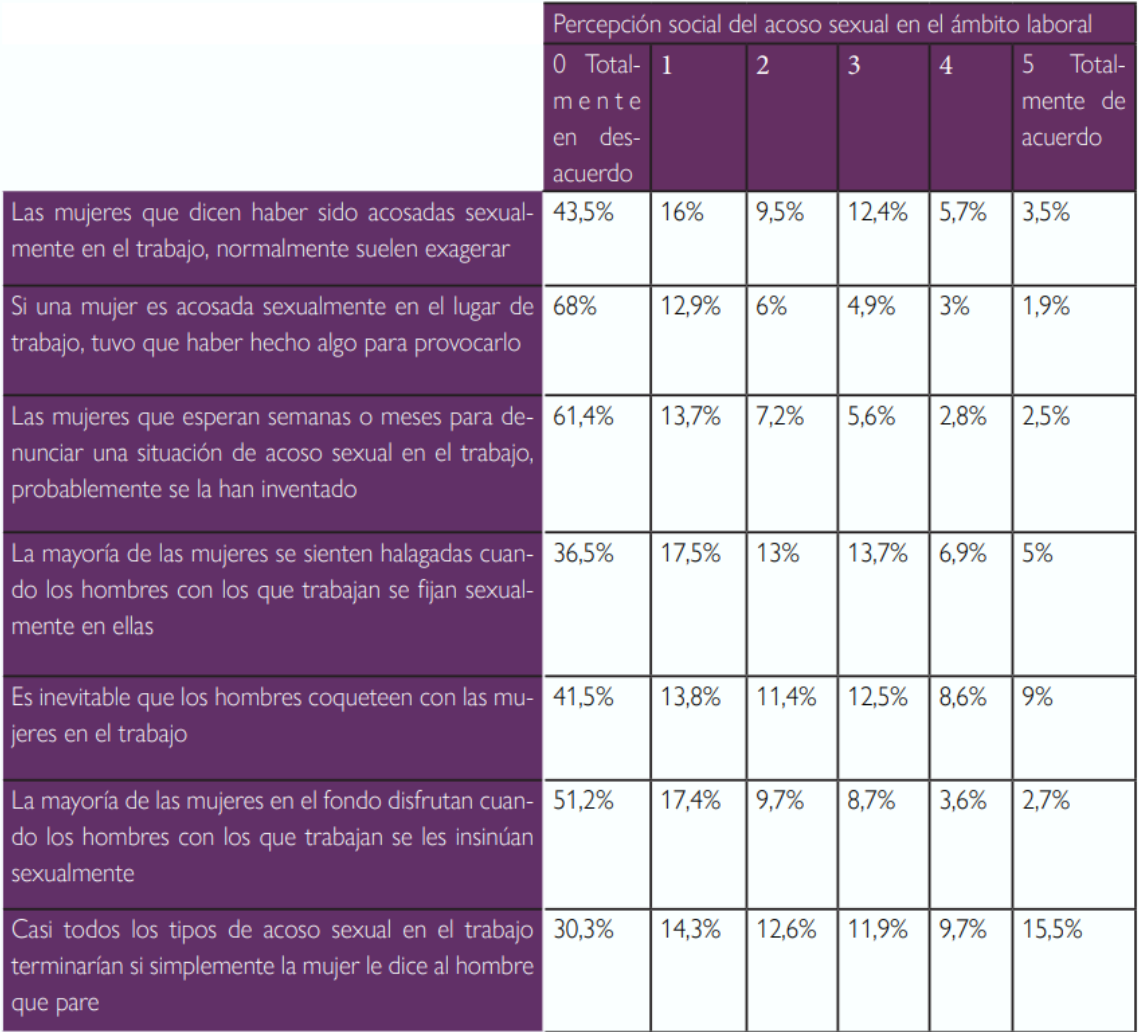
\includegraphics[width=\textwidth]{assets/encuesta_percepcion_social.png}
            \end{figure}
        \end{columns}
    \end{frame}

    \subsection{Perfil de víctima y acosador/a}

    \begin{frame}
        \frametitle{Perfil de víctima y acosador/a}
        \begin{columns}
            \column{0.5\textwidth}
            \highlight{Perfil de victima}: Mayoritariamente mujeres, más en grupos vulnerables:
            \begin{itemize}
                \item Solas con responsabilidades familiares
                \item Sectores laborales masculinizados
                \item Jóvenes en su primer trabajo
                \item Discapacidad
                \item Migrantes o de minorías étnicas
                \item Contratos temporales o subcontratadas
            \end{itemize}
            \column{0.5\textwidth}
            \highlight{Perfil de acosador/a}: Mayoritariamente varones
            \begin{itemize}
                \item Superiores jerárquicos, compañeros o clientes
                \item Cualquier estrato social, nivel ocupacional y categoría profesional
                \item No hay un rango de edad específico
                \item Creencias y actitudes sexistas vinculadas a la masculinidad tradicional
            \end{itemize}
        \end{columns}
    \end{frame}

    \subsection{Consecuencias del acoso sexual y acoso por razón de sexo}

    \begin{frame}
        \frametitle{Consecuencias del acoso sexual y acoso por razón de sexo}
        \framesubtitle{Consecuencias sobre la salud}
        \begin{itemize}
        \item \highlight{Estrés crónico}: Desequilibrio entre la demanda percibida del entorno y la capacidad de adaptación del organismo, manifestándose como ansiedad, hostilidad o depresión.
        \begin{itemize}
            \item \highlight{Físicas}: Trastornos coronarios, dermatológicos, endocrinos, gastrointestinales, respiratorios, musculoesqueléticos, inmunológicos.
            \item \highlight{Cognitivas}: Déficit de atención, concentración y memoria, aumento de errores, pensamientos recurrentes.
            \item \highlight{Conductuales}: Sedentarismo, abuso de sustancias, conductas peligrosas, sueño inadecuados, respuestas agresivas, suicidio.
            \item \highlight{Emocionales}: Irritabilidad, ansiedad, temor, fobias, impulsividad, desconfianza, tristeza, apatía, depresión, ira.
            \item \highlight{Sociales}: Aislamiento, conflictos, ausencia de comunicación, evitación, indemnizaciones, publicidad negativa.
            \item \highlight{Organizacionales}: Más absentismo, más accidentes, menor productividad, estancamiento laboral, despidos, responsabilidad legal.
        \end{itemize}
        \end{itemize}
    \end{frame}

    \begin{frame}
        \frametitle{Consecuencias del acoso sexual y acoso por razón de sexo}
        \framesubtitle{Consecuencias del acoso como accidente laboral}
        \begin{itemize}
            \item El acoso sexual es considerado un \highlight{riesgo laboral}
            \item Sus consecuencias deberían considerarse \highlight{accidente de trabajo}
            \item Generalmente se declaran como \highlight{contingencia común}
            \item Para ser considerado accidente de trabajo, se necesita:
            \begin{itemize}
                \item Existencia y acreditación del acoso y del daño
                \item Identificación de nexo causal entre lesión y trabajo
            \end{itemize}
            \item  Determinación de contingencias
            \begin{itemize}
                \item De oficio por el INSS
                \item A instancias del trabajador, su representante legal o las Mutuas de trabajo
            \end{itemize}
        \end{itemize}
    \end{frame}

    \subsection{Asistencia/apoyo a las víctimas de acoso}

    \begin{frame}
        \frametitle{Asistencia/apoyo a las víctimas de acoso}
        \begin{itemize}
        \item ¿Qué puedo hacer si me siento acosada/o?
        \begin{itemize}
        \item \highlight{Solicitar información}: A la empresa sobre procedimientos de actuación, a la representación legal de los trabajadores, al servicio de información y asesoramiento del Instituto de la Mujer
        \item \highlight{Resolución informal del conflicto}: Intentar resolver el conflicto conforme al protocolo de la empresa, garantizando confidencialidad
        \item \highlight{Presentar una denuncia}: Inspección de Trabajo y Seguridad Social, Policía o juzgado de guardia (no anónimas, por la persona afectada)
        \end{itemize}
        \item ¿En qué consiste la asistencia y apoyo a las víctimas?
        \begin{itemize}
            \item Información sobre cómo actuar y derechos
            \item Asistencia psicológica y médica
            \item Asesoramiento jurídico y profesional
            \item Apoyo emocional y acompañamiento
            \item Información sobre medidas disciplinarias y penales
            \item Ejecución de medidas y prevención de represalias
        \end{itemize}
    \end{itemize}
    \end{frame}

    \subsection{Detección temprana del acoso sexual y acoso por razón de sexo}
    \begin{frame}
        \frametitle{AS y ARS como riesgo psicosocial en el ámbito laboral}
        \framesubtitle{Detección temprana del acoso sexual y acoso por razón de sexo}
    \end{frame}

    \subsection{Prevención del acoso sexual y acoso por razón de sexo}
    \begin{frame}
        \frametitle{AS y ARS como riesgo psicosocial en el ámbito laboral}
        \framesubtitle{Prevención del acoso sexual y acoso por razón de sexo}
    \end{frame}

    \subsection{Proyectos}
    \begin{frame}
        \frametitle{AS y ARS como riesgo psicosocial en el ámbito laboral}
        \framesubtitle{Proyectos}
    \end{frame}


    \section{Protocolo frente al acoso sexual y acoso por razón de sexo}

    \subsection{Normativa}
    \begin{frame}
        \frametitle{Protocolo frente al acoso sexual y acoso por razón de sexo}
        \framesubtitle{Normativa}
    \end{frame}

    \subsection{Definiciones}
    \begin{frame}
        \frametitle{Protocolo frente al acoso sexual y acoso por razón de sexo}
        \framesubtitle{Definiciones}
    \end{frame}

    \subsection{Ámbito penal}
    \begin{frame}
        \frametitle{Protocolo frente al acoso sexual y acoso por razón de sexo}
        \framesubtitle{Ámbito penal}
    \end{frame}

    \subsection{Ámbito administrativo}
    \begin{frame}
        \frametitle{Protocolo frente al acoso sexual y acoso por razón de sexo}
        \framesubtitle{Ámbito administrativo}
    \end{frame}

    \subsection{Medidas administrativas en el MICIU}
    \begin{frame}
        \frametitle{Protocolo frente al acoso sexual y acoso por razón de sexo}
        \framesubtitle{Medidas administrativas en el MICIU}
    \end{frame}

    \subsection{Medidas disciplinarias}
    \begin{frame}
        \frametitle{Protocolo frente al acoso sexual y acoso por razón de sexo}
        \framesubtitle{Medidas disciplinarias}
    \end{frame}


    \section{Acoso y violencia de género en el ámbito digital}

    \subsection{Problemas a abordar en violencia digital sexual}
    \begin{frame}
        \frametitle{Acoso y violencia de género en el ámbito digital}
        \framesubtitle{Problemas a abordar en violencia digital sexual. Punto de vista social y criminológico}
    \end{frame}

    \subsection{Dificultades en la investigación de delitos tecnológicos de género}
    \begin{frame}
        \frametitle{Acoso y violencia de género en el ámbito digital}
        \framesubtitle{Dificultades en la investigación de delitos tecnológicos de género}
    \end{frame}

    \subsection{Exigencias de la nueva directiva de violencia}
    \begin{frame}
        \frametitle{Acoso y violencia de género en el ámbito digital}
        \framesubtitle{Exigencias de la nueva directiva de violencia}
    \end{frame}


    \section{}

    \subsection{}

    \begin{frame}
        \begin{block}{}
            \centering
            ¡Gracias por vuestra atención!
        \end{block}
    \end{frame}

\end{document}